\documentclass[12pt,aps,pre]{revtex4}
%\documentclass[aps,pre,onecolumn,superscriptaddress]{revtex4-1}
\usepackage{graphicx, epsfig,cancel}
\usepackage{color}
\usepackage{textcomp}
\usepackage{amssymb,amsmath} 
\usepackage{setspace}

% for writing code snippets in latex
\usepackage{listings}

\definecolor{dkgreen}{rgb}{0,0.6,0}
\definecolor{gray}{rgb}{0.5,0.5,0.5}
\definecolor{mauve}{rgb}{0.58,0,0.82}

\lstset{frame=tb,
  language=C++,
  aboveskip=3mm,
  belowskip=3mm,
  showstringspaces=false,
  columns=flexible,
  basicstyle={\small\ttfamily},
  numbers=none,
  numberstyle=\tiny\color{gray},
  keywordstyle=\color{blue},
  commentstyle=\color{dkgreen},
  stringstyle=\color{mauve},
  breaklines=true,
  breakatwhitespace=true,
  tabsize=3
}

\newcommand{\blue}[1]{\textcolor{blue}{#1}}
\newcommand{\red}[1]{\textcolor{red}{[#1]}}
\newcommand{\green}[1]{\textcolor{green}{#1}}

\begin{document}
\setstretch{1.5}
\title{Multi-Scale Formulation for Biotissue Code}
\author{V. W. L. Chan}
\maketitle

\section{Macro-scale}

\subsection{Weak Formulation}
We are interested in solving the following strong-form problem on the macroscale
%
\begin{align}
&\nabla \cdot \pmb{\sigma} = 0 \ \text{ on } \ \Omega \nonumber\\
&\pmb{\sigma} \cdot \pmb{n} = \bar{\pmb{t}} \ \text{ on } \ \Gamma_t \nonumber\\
&\pmb{u} = \bar{\pmb{u}} \ \text{ on } \ \Gamma_u 
\label{eq:strong_form}
\end{align}
%
where $\bar{\pmb{t}}$ and $\bar{\pmb{u}}$ are prescribed traction and displacements, respectively, and $\pmb{\sigma}$ is the Cauchy stress tensor
%
\begin{eqnarray}
[\pmb{\sigma}] \equiv
\begin{bmatrix}
\sigma_{11} & \sigma_{12} & \sigma_{13} \\
\sigma_{21} & \sigma_{22} & \sigma_{23} \\
\sigma_{31} & \sigma_{32} & \sigma_{33} 
\end{bmatrix} .
\label{eq:Cauchy_stress_tensor}
\end{eqnarray}
%
Since we are using the finite-element method (FEM), we will need to consider the weak form of Eq.\ \eqref{eq:strong_form}. The weak form can be obtained by multiplying both sides by an admissible test function $\phi$ and integrating over the domain:
%
\begin{align}
&\int_{\Omega} \phi (\nabla \cdot \pmb{\sigma})d\Omega  = 0 \ \ \forall \phi \in U_0 \nonumber\\
&\int_{\Gamma_t}\phi (\bar{\pmb{t}}-\pmb{\sigma} \cdot \pmb{n})d\Gamma_t = 0 \ \ \forall \phi \in U_0 \nonumber\\
&U_0 = \{\phi \mid \phi \in H^1, \phi = 0 \ \text{ on } \Gamma_u \} .
\label{eq:weak_form1}
\end{align}
%

Next we apply the product rule and divergence theorem:
%
\begin{equation}
\nabla \cdot (\phi \pmb{\sigma}) = \pmb{\sigma} \nabla \phi + \phi (\nabla \cdot \pmb{\sigma})\ \text{ and } \ \int_{\Omega} \nabla \cdot \textbf{F} d\Omega = \int_{\Gamma} \textbf{F} \cdot \textbf{n} d\Gamma,
\end{equation}
%
respectively, to the first relationship in Eq.\ \eqref{eq:weak_form1} to obtain
%
\begin{eqnarray}
\int_{\Omega} \phi (\nabla \cdot \pmb{\sigma})d\Omega &=&\int_{\Omega} \nabla \cdot (\phi \pmb{\sigma}) d\Omega - \int_{\Omega} \pmb{\sigma} \nabla \phi d\Omega \nonumber\\
%
&=& \int_{\Gamma} (\phi \pmb{\sigma}) \cdot \pmb{n} d\Gamma - \int_{\Omega} \pmb{\sigma} \nabla \phi d\Omega .
\end{eqnarray}
%
Note that we have applied the product rule in the first line and the divergence theorem in the second line. Using the above relationship, Eq.\ \eqref{eq:weak_form1} becomes
%
\begin{align}
&\int_{\Omega} \pmb{\sigma} \nabla \phi d\Omega = \int_{\Gamma} (\phi \pmb{\sigma}) \cdot \pmb{n} d\Gamma = \int_{\Gamma} \phi \bar{\pmb{t}} d\Gamma \ \ \forall \phi \in U_0 \nonumber\\
 &U_0 = \{\phi \mid \phi \in H^1, \phi = 0 \ \text{ on } \Gamma_u \} .
\label{eq:weak_form}
\end{align}
%
Note that we have not used a constitutive relation to define $\pmb{\sigma}$ in terms of displacements. As shown later on, the values of $\pmb{\sigma}$ are obtained from the microscale.

\subsection{Newton-Raphson Method and the Tangent-Stiffness Matrix}

The Newton-Raphson procedure for solving a nonlinear set of equations is [Bonet and Wood]
%
\begin{eqnarray}
\pmb{K}(\pmb{u}^k) \delta \pmb{u} = - \pmb{R}(\pmb{u}^k), \ \pmb{u}^{k+1} = \pmb{u}^k + \delta \pmb{u},
\label{eq:Newton-Raphson}
\end{eqnarray}
%
where $\pmb{R}$ is the out-of-balance force, $\pmb{K}$ is the tangent stiffness matrix, and the superscript $k$ indicates the pseudo time step of the procedure. The left-hand-side of  Eq.\ \eqref{eq:Newton-Raphson} is determined from the directional derivative of $\pmb{R}$ with respect to $\pmb{u}^k$ and in the direction of $\delta \pmb{u}$:
%
\begin{eqnarray}
\pmb{K}(\pmb{u}^k) \delta \pmb{u} &=& D\pmb{R}(\pmb{u}^k)[\pmb{u}] \nonumber\\
%
&=& \frac{d}{d\epsilon} \bigg|_{\epsilon=0}\pmb{R}(\pmb{u}^k + \epsilon \delta \pmb{u}) \nonumber\\
&=& \frac{d \pmb{R}}{d\pmb{u}^k} \frac{d(\pmb{u}^k + \epsilon \delta \pmb{u})}{d\epsilon} \bigg|_{\epsilon=0} \nonumber\\
&=& \frac{d \pmb{R}}{d\pmb{u}^k} \delta \pmb{u}.
\label{eq:DR[u]}
\end{eqnarray}
%
In matrix form we have
%
\begin{eqnarray}
[\pmb{K}(\pmb{u}^k)][\delta \pmb{u}] =
%
\begin{bmatrix}
\frac{\partial R_1}{\partial u_1^k} & \frac{\partial R_1}{\partial u_2^k} & \frac{\partial R_1}{\partial u_3^k} \\
%
\frac{\partial R_2}{\partial u_1^k} & \frac{\partial R_2}{\partial u_2^k} & \frac{\partial R_2}{\partial u_3^k} \\
%
\frac{\partial R_3}{\partial u_1^k} & \frac{\partial R_3}{\partial u_2^k} & \frac{\partial R_3}{\partial u_3^k} \\
\end{bmatrix}
%
\begin{bmatrix}
\delta u_1 \\ \delta u_2 \\ \delta u_3
\end{bmatrix}, \ \ \text{where} \ \ 
%
[\pmb{R}] = 
\begin{bmatrix}
R_1 \\ R_2 \\ R_3
\end{bmatrix}.
\label{eq:DR[u]_matrix}
\end{eqnarray}
%

To apply the Newton-Raphson procedure to our problem of interest, $\pmb{R}$ is defined in terms of Eq.\ \eqref{eq:weak_form}:
%
\begin{align}
&\pmb{R} = \int_{\Omega} \pmb{\sigma} \nabla \phi d\Omega - \int_{\Gamma} \phi \bar{\pmb{t}} d\Gamma \ \ \forall \phi \in U_0 \nonumber\\
&U_0 = \{\phi \mid \phi \in H^1, \phi = 0 \ \text{ on } \Gamma_u \} .
\label{eq:R}
\end{align}
% 
Equation \eqref{eq:R} can also be written in matrix form
%
\begin{eqnarray}
[\pmb{R}] = \int_{\Omega} [\pmb{\sigma}] [\nabla \phi] d\Omega - \int_{\Gamma} \phi [\bar{\pmb{t}}] d\Gamma, \ \ \text{where} \ \
%
[\nabla \phi] \equiv 
\begin{bmatrix}
\frac{\partial \phi}{\partial x_1} \\ \frac{\partial \phi}{\partial x_2} \\ \frac{\partial \phi}{\partial x_3}
\end{bmatrix}  \ \text{and} \ \ 
%
[\bar{\pmb{t}}] \equiv 
\begin{bmatrix}
\bar{t}_1 \\ \bar{t}_2 \\ \bar{t}_3
\end{bmatrix},
%
\label{eq:R_matrix}
\end{eqnarray}
%
as well as with index notation as 
%
\begin{equation}
R_i = \int_{\Omega}\sigma_{ij} \frac{\partial \phi}{\partial x_j} d\Omega - \int_{\Gamma} \phi \bar{t}_i d\Gamma,
\label{eq:R_index}
\end{equation}
%
where repeated indices are summed. 

As seen in Eq.\ \eqref{eq:DR[u]_matrix} the tangent-stiffness matrix is calculated from the derivatives of $\pmb{R}$. Since the elements of $\pmb{R}$ are integral equations (c.f., Eq.\ \ref{eq:R_index}), we apply the Leibniz integration rule (\red{Actually need to apply the Reynold's Transport Theorem here because integration bounds change as system is deformed}),
%
\begin{equation}
\frac{\partial}{\partial x}\left(\int_{y_0}^{y_1} f(x,y) dy \right) = \int_{y_0}^{y_1} \frac{\partial f(x,y)}{\partial x} dy,
\label{eq:leibniz}
\end{equation}
%
to express the tangent-stiffness matrix in terms of the Cauchy stress and the derivatives of the Cauchy stress and test function. Each element of the tangent-stiffness matrix is expressed in index notation as
%
\begin{eqnarray}
[\pmb{K}(\pmb{u}^k)]_{ij} \equiv \frac{\partial R_i}{\partial u_j^k} &=& \int_{\Omega} \frac{\partial \sigma_{il}}{\partial u_j^k} \frac{\partial \phi}{\partial x_l}  +  \sigma_{il} \frac{\partial}{\partial u_i^k}\frac{\partial \phi}{\partial x_l} d\Omega - \int_{\Gamma} \bar{t}_i \frac{\partial \phi}{\partial u_j^k} d\Gamma .
\label{eq:tangent-stiffness_index}
\end{eqnarray}
%

The derivatives of $\phi$ in Eq.\ \eqref{eq:tangent-stiffness_index}:
%
\begin{equation}
\frac{\partial \phi}{\partial x_l}, \ \ \frac{\partial}{\partial u_i^k}\frac{\partial \phi}{\partial x_l}, \ \text{and} \ \frac{\partial \phi}{\partial u_j^k}, 
\label{eq:phi_terms}
\end{equation}
%
are evaluated using linear tetrahedral shape functions, while the Cauchy stresses and their derivatives:
%
\begin{equation}
\sigma_{il} \ \text{and} \ \frac{\partial \sigma_{il}}{\partial u_j^k},
\label{eq:sigma_terms}
\end{equation}
%
are evaluated from calculations at the microscale representative volume elements (RVEs).

\section{Micro-scale}
%
\subsection{Cauchy Stress}
%
According to [Stylianopolous and Barocas] an element of the Cauchy stress tensor can be obtained from a volume-averaging technique
%
\begin{equation}
\sigma_{ij} = \frac{1}{V} \sum_{n \in bcl} x_i^{n} T_j^{n} 
\label{eq:cauchy_stress_element}
\end{equation}
%
where $V$ is the current volume of the RVE, $x_i^{n}$ is the $i^{th}$ coordinate of the cross-link on the boundary of the RVE ($bcl$), and $T_j^{n}$ is the $j^{th}$ component of the internal force of a cross-link on the boundary. 
%
\subsection{Cauchy-Stress Derivative}
%
The derivative of the Cauchy stress is evaluated by using Eq.\ \eqref{eq:cauchy_stress_element} and applying the chain rule
%
\begin{eqnarray}
\frac{\partial \sigma_{ij}}{\partial  u^k_m}  &=& \frac{\partial \sigma_{ij}}{\partial x_l^{\text{RVE}}} \frac{\partial x_l^{\text{RVE}}}{\partial u^k_m} \nonumber\\
%
&=& \left [ \frac{\partial}{\partial x^{\text{RVE}}_l}  \left(\frac{1}{V} \sum_{n \in bcl} x_i^{n} T_j^{n}\right)+ \frac{1}{V} \frac{\partial}{\partial x^{\text{RVE}}_l} \left(\sum_{n \in bcl} x_i^{n} T_j^{n} \right) \right] \frac{\partial x_l^{\text{RVE}}}{\partial u^k_m} \nonumber\\
%
&=&  \left[\frac{\partial}{\partial x^{\text{RVE}}_l}  \left(\frac{s_{ij}}{V} \right) + \frac{1}{V} \frac{\partial s_{ij}}{\partial x^{\text{RVE}}_l}\right]\frac{\partial x_l^{\text{RVE}}}{\partial u^k_m} \nonumber\\
%
&=& \left[\frac{1}{V} \frac{\partial s_{ij}}{\partial x^{\text{RVE}}_l} -\frac{1}{V^2}\frac{\partial V}{\partial x^{\text{RVE}}_l}s_{ij} \right]\frac{\partial x_l^{\text{RVE}}}{\partial u^k_m},
\end{eqnarray}
%
where $x_l^{\text{RVE}}$ are the RVE corner coordinates and $s_{ij} \equiv \sum_{n \in bcl} x^n_i T^n_j$. Since our RVE is a hexahedron, the subscript $l$ ranges from 1 to 24; 8 corner nodes $\times$ 3 degrees of freedom per corner node.  Therefore, the calculation of the stress derivatives involves the calculation of three different derivatives:
%
\begin{equation}
\frac{\partial s_{ij}}{\partial x_l^{\text{RVE}} }, \ \
\frac{\partial V}{\partial x_l^{\text{RVE}}}, \ \ \text{ and } \ \ 
\frac{\partial x_l^{\text{RVE}}}{\partial u^k_m}
\end{equation}
%
\subsubsection{Derivative of $s_{ij}$ with respect to RVE corner coordinates}
%
Applying the chain rule, the derivative of $s_{ij}$ can be written as
%
\begin{eqnarray}
\frac{\partial s_{ij}}{\partial x_l^{\text{RVE}}} &=& \frac{\partial s_{ij}}{\partial x_k}\frac{\partial x_k}{\partial x_l^{\text{RVE}}} \nonumber\\ 
%
&=& \frac{\partial}{\partial x_k} \left(\sum_{n \in bcl} x_i^{n} T_j^n \right) \frac{\partial x_k}{\partial x_l^{\text{RVE}}} \nonumber\\
%
&=&\sum_{n \in bcl} \left( \frac{\partial x_i^{n}}{\partial x_k} T_j^n + x_i^n \frac{\partial T_j^n}{\partial x_k}  \right) \frac{\partial x_k}{\partial x_l^{\text{RVE}}} \nonumber\\
%
&=&\sum_{n \in bcl} \left( \delta_{ik} T_j^n + x_i^n \frac{\partial T_j^n}{\partial x_k}  \right) \frac{\partial x_k}{\partial x_l^{\text{RVE}}}
\label{eq:dsdxRVE}
\end{eqnarray}
%
where $x_k$ is the $k^{th}$ coordinate of the fiber nodes in the RVE; the subscript $k$ ranges from 1 to $N_{dof}^{fn} \equiv 3 \ dofs \ \times$ number of fiber nodes. Since $\frac{\partial T_j^n}{\partial x_k}$ is the $(j,k)^{th}$ element of the tangent-stiffness matrix for cross-links on the boundary, the terms within the parenthesis in Eq.\ \eqref{eq:dsdxRVE} are available from the force balance of the fiber network in the RVE. 

At this point, we still need to determine the derivative of fiber-node coordinates of the RVE $(x_k)$ with respect to the corner-node coordinates of the RVE $(x_l^{RVE})$. A relationship between $x_k$ and $x_l^{RVE}$ is obtained by considering how the internal fiber forces (i.e., the residual on fiber network) changes with respect to $x_l^{RVE}$ (i.e., the displacements at the RVE corner nodes):
%
\begin{equation}
\frac{\partial \pmb{R}}{\partial \pmb{x}^{RVE}} = \frac{\partial \pmb{R}}{\partial \pmb{x}^{RVE}} \bigg |_{\pmb{x}} + \frac{\partial \pmb{R}}{\partial \pmb{x}} \bigg |_{\pmb{x}^{RVE}} \frac{\partial \pmb{x}}{\partial \pmb{x}^{RVE}},
\label{eq:dRdxRVE}
\end{equation}
%
where
%
\begin{eqnarray}
\pmb{R} \equiv \begin{bmatrix}
T_1 \\
T_2 \\
\vdots \\
T_{N_{dof}^{fn}}
\end{bmatrix}, \ \ 
%
\pmb{x}^{RVE} \equiv \begin{bmatrix}
x_1^{RVE} \\
x_2^{RVE} \\
\vdots \\
x_{24}^{RVE}
\end{bmatrix}, \ \text{and} \
%
\pmb{x} \equiv \begin{bmatrix}
x_1 \\
x_2 \\
\vdots \\
x_{N_{dof}^{fn}} 
\end{bmatrix} .
\end{eqnarray}
%
In Eq.\ \eqref{eq:dRdxRVE} the change in residual with respect to $\pmb{x}^{RVE}$ has 2 contributions: change due to (1) RVE corner-node displacements when interior-nodes are fixed and (2) interior-node displacements when RVE corner-nodes  are fixed. When the forces in the fiber network are balanced, $\partial \pmb{R}/\partial \pmb{x}^{RVE} = 0$, and the derivative $\partial \pmb{x}/\partial \pmb{x}^{RVE}$ needed to evaluate Eq.\ \eqref{eq:dsdxRVE} can be determined by
%
\begin{equation}
\frac{\partial \pmb{x}}{\partial \pmb{x}^{RVE}} = -\left(\frac{\partial \pmb{R}}{\partial \pmb{x}} \bigg |_{\pmb{x}^{RVE}}\right)^{-1}\frac{\partial \pmb{R}}{\partial \pmb{x}^{RVE}}\bigg |_{\pmb{x}} .
\end{equation}
%
Since $\partial \pmb{R}/\partial \pmb{x} |_{\pmb{x}^{RVE}}$ is the tangent-stiffness matrix, $\partial \pmb{x}/\partial \pmb{x}^{RVE}$ can be determined once $\partial \pmb{R}/\partial \pmb{x}^{RVE} |_{\pmb{x}}$ is known. Note that the inverse of the tangent-stiffness matrix has already been evaluated when performing the Newton-Raphson procedure for balancing the force of the fiber network.

The change of residual with respect to $\pmb{x}^{RVE}$ while the interior nodes are fixed is calculated by a geometric argument. To illustrate this calculation, consider a single fiber node that lies on the boundary of the RVE box 
%
\begin{align}
&\left [\frac{\partial \pmb{R}}{\partial \pmb{x}^{RVE}}\bigg |_{\pmb{x}}\right] = \nonumber\\
%
&\begin{bmatrix} 
\frac{\partial T_1}{\partial x_1^{RVE}} & \frac{\partial T_1}{\partial x_2^{RVE}} & \frac{\partial T_1}{\partial x_3^{RVE}} & \cdots & \frac{\partial T_1}{\partial x_{22}^{RVE}} & \frac{\partial T_1}{\partial x_{23}^{RVE}} & \frac{\partial T_1}{\partial x_{24}^{RVE}} \\
%
\frac{\partial T_2}{\partial x_1^{RVE}} & \frac{\partial T_2}{\partial x_2^{RVE}} & \frac{\partial T_2}{\partial x_3^{RVE}} & \cdots & \frac{\partial T_2}{\partial x_{22}^{RVE}} & \frac{\partial T_2}{\partial x_{23}^{RVE}} & \frac{\partial T_2}{\partial x_{24}^{RVE}} \\
%
\frac{\partial T_3}{\partial x_1^{RVE}} & \frac{\partial T_3}{\partial x_2^{RVE}} & \frac{\partial T_3}{\partial x_3^{RVE}} & \cdots & \frac{\partial T_3}{\partial x_{22}^{RVE}} & \frac{\partial T_3}{\partial x_{23}^{RVE}} & \frac{\partial T_3}{\partial x_{24}^{RVE}} \\
\end{bmatrix} \nonumber\\
%
& \begin{bmatrix}
\frac{A_1}{A}\pmb{I}_{3\times3} & \cdots & \frac{A_8}{A}\pmb{I}_{3\times3}
\end{bmatrix},
\label{eq:dRdxRVE_1node}
\end{align}
%
where $A$ is the total area of the face on which the fiber node lies and $A_i$ is the portion of the RVE face enclosed by the fiber node and the $i^{th}$ RVE corner node; $A_i$ is nonzero only for fiber nodes that lie on one of the RVE faces. See Fig.\ \ref{fig:dRdxRVE} for a schematic of $A_i/A$. To form the full of $\partial \pmb{R}/\partial \pmb{x}^{RVE} |_{\pmb{x}}$, every fiber node must be considered. Since each fiber node contributes three rows to the matrix, the dimensions of $\partial \pmb{R}/\partial \pmb{x}^{RVE} |_{\pmb{x}}$ is $3 \ \times N_{dof}^{fn}$ by 24 (number of RVE corner nodes $\times$ 3 dofs per corner node).
%
\begin{figure}[ht]
\begin{center}$
\begin{array}{cc}
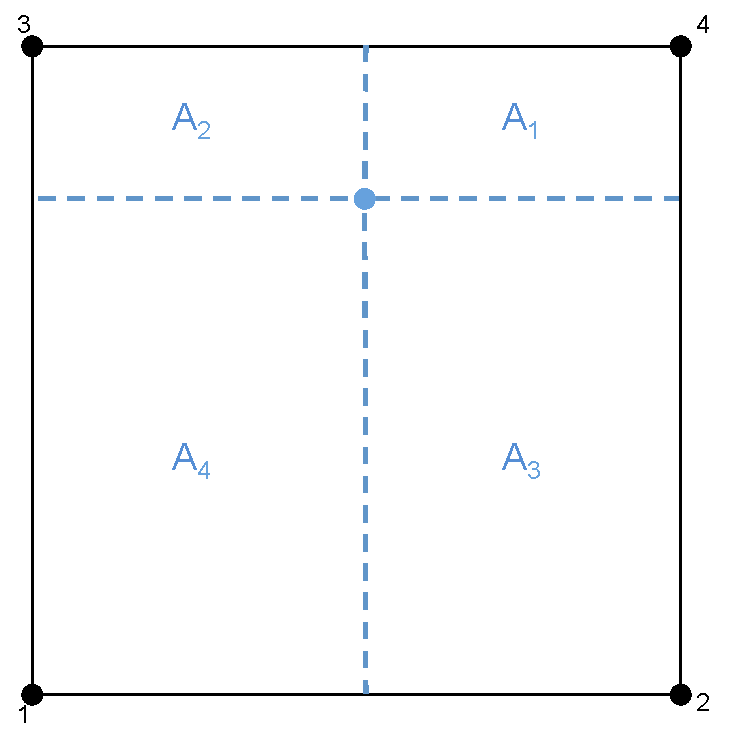
\includegraphics[height=2.5in]{dRdxRVE.pdf}
\end{array}$
\end{center}
\caption{Two-dimensional schematic of $A_i/A$. Blue dot represents fiber node that lies on RVE face. Black dots represent the 4 nodes on an RVE face. The total area of the RVE face is $A=A_1+A_2+A_3+A_4$. }
\label{fig:dRdxRVE}
\end{figure}
%
\subsubsection{Derivative of $V$ with respect to RVE corner coordinates}

The volume can be calculated in the parent domain by
%
\begin{equation}
V = \int_{-1}^{1} \int_{-1}^1 \int_{-1}^1 \text{det}\pmb{J}^e d\xi_1 d\xi_2 d\xi_3  = \int_{-1}^{1} \left(\int_{-1}^1 \left(\int_{-1}^1 \text{det}\pmb{J}^e d\xi_1 \right)d\xi_2\right) d\xi_3 ,
\label{eq:volume}
\end{equation}
%
which has been written in terms of three consecutive integrals. In the biotissue code, the integrals are evaluated using the Gauss integration formula where Eq.\ \eqref{eq:volume} becomes 
%
\begin{equation}
V = \sum_{i=1}^{N_{gp}} \sum_{j=1}^{N_{gp}} \sum_{k=1}^{N_{gp}} W_i W_j W_k \text{det}\pmb{J}^e(\xi_1^{(i)},\xi_2^{(j)},\xi_3^{(k)})
\label{eq:gauss_integration}
\end{equation}
%
where $N_{gp}$ is the number of Gauss integration points, $W_i$ is the weight of the $i^{th}$ integration point, $\pmb{J}^e$ is the Jacobian matrix, and $\xi_i^{(j)}$ is the $i^{th}$ component of the $j^{th}$ integration point. Note that $V$ is the volume for a hexahedron where $N_{gp}=2$, $W_i=1$, and $\xi_i^{(j)}=\pm 1/\sqrt{3}$. 

The derivative of the Volume with respect to the RVE corner coordinates can be written in index notation as
%
\begin{eqnarray}
\frac{\partial V}{\partial x_l^{RVE}} &=& \int_{-1}^1 \int_{-1}^1 \int_{-1}^1 \frac{\partial}{\partial x_l^{RVE}} \left(\text{det}\pmb{J}^e\right) d\xi_1 d\xi_2 d\xi_3 \nonumber\\
%
&=& \sum_{i=1}^{N_{gp}} \sum_{j=1}^{N_{gp}} \sum_{k=1}^{N_{gp}} W_i W_j W_k \frac{\partial}{\partial x_l^{RVE}} \left(\text{det}\pmb{J}^e(\xi_1^{(i)},\xi_2^{(j)},\xi_3^{(k)})\right),
\label{eq:dVdvl}
\end{eqnarray}
%
where we have applied the Gauss integration formula (c.f., Eq.\ \eqref{eq:gauss_integration}). The derivative of det$\pmb{J}^e(\xi_1^{(i)},\xi_2^{(j)},\xi_3^{(k)})$ is 
%
\begin{eqnarray}
&&\frac{\partial}{\partial x_l^{RVE}}\left(\text{det}\pmb{J}^e(\xi_1^{(i)},\xi_2^{(j)},\xi_3^{(k)})\right) \nonumber\\
%
&&= \frac{\partial}{\partial x_l^{RVE}}\bigg[x_{,\xi_1}\left(y_{,\xi_2}z_{,\xi_3} - z_{,\xi_2}y_{,\xi_3} \right) - y_{,\xi_1}\left(x_{,\xi_2}z_{,\xi_3}-z_{,\xi_2}x_{,\xi_3} \right) + z_{,\xi_1}\left(x_{,\xi_2}y_{,\xi_3}-y_{,\xi_2}x_{,\xi_3} \right)\bigg] \bigg |_{\xi_1 = \xi_1^{(i)}, \xi_2 = \xi_2^{(j)}, \xi_3 = \xi_3^{(k)}}.  \nonumber\\
\end{eqnarray}
%
To illustrate, the $x, y, z$ components of the derivative for the ``first" node of the hexahedron $(x_1^{RVE},x_2^{RVE}, x_3^{RVE})$ are explicitly written out:
%
\begin{eqnarray}
\frac{\partial \text{det}\pmb{J}^e}{\partial x_1^{RVE}} &=& \frac{\partial x_{,\xi_1}}{\partial x_1^{RVE}}\left(y_{,\xi_2}z_{,\xi_3} - z_{,\xi_2}y_{,\xi_3} \right) - y_{,\xi_1}\left(\frac{\partial x_{,\xi_2}}{\partial x_1^{RVE}}z_{,\xi_3}-z_{,\xi_2}\frac{\partial x_{,\xi_3}}{\partial x_1^{RVE}} \right) + z_{,\xi_1}\left(x_{,\xi_2}y_{,\xi_3}-y_{,\xi_2}x_{,\xi_3} \right) \nonumber\\
%
&=& \text{det} \begin{bmatrix}
\frac{\partial x_{,\xi_1}}{\partial x_1^{RVE}} & y_{,\xi_1} & z_{,\xi_1} \\
\frac{\partial x_{,\xi_2}}{\partial x_1^{RVE}} & y_{,\xi_2} & z_{,\xi_2} \\
\frac{\partial x_{,\xi_3}}{\partial x_1^{RVE}} & y_{,\xi_3} & z_{,\xi_3}
\end{bmatrix} 
%
= \text{det} \begin{bmatrix}
\frac{\partial N_1^{6\text{hex}}}{\partial \xi_1} & y_{,\xi_1} & z_{,\xi_1} \\
\frac{\partial N_1^{6\text{hex}}}{\partial \xi_2} & y_{,\xi_2} & z_{,\xi_2} \\
\frac{\partial N_1^{6\text{hex}}}{\partial \xi_3} & y_{,\xi_3} & z_{,\xi_3}
\end{bmatrix} \nonumber\\
%%
\frac{\partial \text{det}\pmb{J}^e}{\partial x_2^{RVE}} &=& x_{,\xi_1}\left(\frac{\partial y_{,\xi_2}}{\partial x_2^{RVE}}z_{,\xi_3} - z_{,\xi_2}\frac{\partial y_{,\xi_3}}{\partial x_2^{RVE}} \right) - \frac{\partial y_{,\xi_1}}{\partial x_2^{RVE}}\left(x_{,\xi_2}z_{,\xi_3}-z_{,\xi_2}x_{,\xi_3} \right) + z_{,\xi_1}\left(x_{,\xi_2}\frac{\partial y_{,\xi_3}}{\partial x_2^{RVE}}-\frac{\partial y_{,\xi_2}}{\partial x_2^{RVE}}x_{,\xi_3} \right) \nonumber\\
%
&=& \text{det} \begin{bmatrix}
x_{,\xi_1} & \frac{\partial y_{,\xi_1}}{\partial x_2^{RVE}} & z_{,\xi_1} \\
x_{,\xi_2} & \frac{\partial y_{,\xi_2}}{\partial x_2^{RVE}} & z_{,\xi_2} \\
x_{,\xi_3} & \frac{\partial y_{,\xi_3}}{\partial x_2^{RVE}} & z_{,\xi_3}
\end{bmatrix} 
%
= \text{det} \begin{bmatrix}
x_{,\xi_1} & \frac{\partial N_2^{6\text{hex}}}{\partial \xi_1} & z_{,\xi_1} \\
x_{,\xi_2} & \frac{\partial N_2^{6\text{hex}}}{\partial \xi_2} & z_{,\xi_2} \\
x_{,\xi_3} & \frac{\partial N_2^{6\text{hex}}}{\partial \xi_3} &  z_{,\xi_3}
\end{bmatrix} \nonumber\\
%%
\frac{\partial \text{det}\pmb{J}^e}{\partial x_3^{RVE}} &=& x_{,\xi_1}\left(y_{,\xi_2} \frac{\partial z_{,\xi_3}}{\partial x_3^{RVE}} - \frac{\partial z_{,\xi_2}}{\partial x_3^{RVE}} y_{,\xi_3} \right) - y_{,\xi_1}\left(x_{,\xi_2}\frac{\partial z_{,\xi_3}}{\partial x_3^{RVE}} - \frac{\partial z_{,\xi_2}}{\partial x_3^{RVE}} x_{,\xi_3} \right) + \frac{\partial z_{,\xi_1}}{\partial x_3^{RVE}}\left(x_{,\xi_2}y_{,\xi_3}-y_{,\xi_2}x_{,\xi_3} \right) \nonumber\\
%
&=& \text{det} \begin{bmatrix}
x_{,\xi_1} & y_{,\xi_1} & \frac{\partial z_{,\xi_1}}{\partial x_2^{RVE}}  \\
x_{,\xi_2} & y_{,\xi_2} & \frac{\partial z_{,\xi_2}}{\partial x_2^{RVE}}  \\
x_{,\xi_3} & y_{,\xi_3} & \frac{\partial z_{,\xi_3}}{\partial x_2^{RVE}} 
\end{bmatrix} 
%
= \text{det} \begin{bmatrix}
x_{,\xi_1} & z_{,\xi_1} & \frac{\partial N_3^{6\text{hex}}}{\partial \xi_1}  \\
x_{,\xi_2} & z_{,\xi_2} & \frac{\partial N_3^{6\text{hex}}}{\partial \xi_2}  \\
x_{,\xi_3} & z_{,\xi_3}& \frac{\partial N_3^{6\text{hex}}}{\partial \xi_3} 
\end{bmatrix} .
\label{eq:ddetJdvl}
\end{eqnarray}
%
Note that the formula for the derivatives for each component of the ``second" to ``eighth" nodes of the hexahedron are essentially the same, with the only difference being the shape function: $N_{l}^{6\text{hex}}$ with $l=4$ to $24$ for components corresponding to the second to eighth nodes. The relationship $\partial x_{,\xi_i}/\partial x_j^{RVE} = \partial N_j^{6\text{hex}}/\partial \xi_i$ was used in Eq.\ \eqref{eq:ddetJdvl}.

\subsubsection{Derivative of RVE corner coordinates with respect to finite-element displacements}

The matrix $[\partial \pmb{x}^{RVE}/\partial \pmb{u}^k]$ has dimensions of 24 (8 RVE corner nodes $\times$ 3 dofs per node) $\times$ 12 (4 FE tetrahedron nodes $\times$ 3 dofs per node) for each element: 
%
\setcounter{MaxMatrixCols}{12}
\begin{eqnarray}
\bigg[ \frac{\partial \pmb{x}^{RVE}}{\partial \pmb{u}^k} \bigg] &=& 
\begin{bmatrix}
\frac{\partial x_1^{RVE}}{\partial u_1^k} & \frac{\partial x_1^{RVE}}{\partial u_2^k} & \frac{\partial x_1^{RVE}}{\partial u_3^k} & &
%
 \frac{\partial x_1^{RVE}}{\partial u_{10}^k} & \frac{\partial x_1^{RVE}}{\partial u_{11}^k} & \frac{\partial x_1^{RVE}}{\partial u_{12}^k} \\
%%%
\frac{\partial x_2^{RVE}}{\partial u_1^k} & \frac{\partial x_2^{RVE}}{\partial u_2^k} & \frac{\partial x_2^{RVE}}{\partial u_3^k} & \cdots &
%
\frac{\partial x_2^{RVE}}{\partial u_{10}^k} & \frac{\partial x_2^{RVE}}{\partial u_{11}^k} & \frac{\partial x_2^{RVE}}{\partial u_{12}^k} \\
%%%
\frac{\partial x_3^{RVE}}{\partial u_1^k} & \frac{\partial x_3^{RVE}}{\partial u_2^k} & \frac{\partial x_3^{RVE}}{\partial u_3^k} &  &
%
\frac{\partial x_3^{RVE}}{\partial u_{10}^k} & \frac{\partial x_3^{RVE}}{\partial u_{11}^k} & \frac{\partial x_3^{RVE}}{\partial u_{12}^k} \\
%%%
 & \vdots & & & & \vdots & \\
 %%%
\frac{\partial x_{22}^{RVE}}{\partial u_1^k} & \frac{\partial x_{22}^{RVE}}{\partial u_2^k} & \frac{\partial x_{22}^{RVE}}{\partial u_3^k} & &
%
 \frac{\partial x_{22}^{RVE}}{\partial u_{10}^k} & \frac{\partial x_{22}^{RVE}}{\partial u_{11}^k} & \frac{\partial x_{22}^{RVE}}{\partial u_{12}^k} \\
%%%
\frac{\partial x_{23}^{RVE}}{\partial u_1^k} & \frac{\partial x_{23}^{RVE}}{\partial u_2^k} & \frac{\partial x_{23}^{RVE}}{\partial u_3^k} & \cdots &
%
\frac{\partial x_{23}^{RVE}}{\partial u_{10}^k} & \frac{\partial x_{23}^{RVE}}{\partial u_{11}^k} & \frac{\partial x_{23}^{RVE}}{\partial u_{12}^k} \\
%%%
\frac{\partial x_{24}^{RVE}}{\partial u_1^k} & \frac{\partial x_{24}^{RVE}}{\partial u_2^k} & \frac{\partial x_{24}^{RVE}}{\partial u_3^k} &  &
%
\frac{\partial x_{24}^{RVE}}{\partial u_{10}^k} & \frac{\partial x_{24}^{RVE}}{\partial u_{11}^k} & \frac{\partial x_{24}^{RVE}}{\partial u_{12}^k} \\
\end{bmatrix} \nonumber\\
%
&=&\begin{bmatrix}
\Delta N_1^{(1)} \pmb{I}_{3\times3} & \Delta N_2^{(1)}\pmb{I}_{3\times3} & \Delta N_3^{(1)} \pmb{I}_{3\times3} & \Delta N_4^{(1)}\pmb{I}_{3\times3} \\
%
\Delta N_1^{(2)} \pmb{I}_{3\times3} & \Delta N_2^{(2)}\pmb{I}_{3\times3} & \Delta N_3^{(2)} \pmb{I}_{3\times3} & \Delta N_4^{(2)}\pmb{I}_{3\times3} \\
%
\Delta N_1^{(3)} \pmb{I}_{3\times3} & \Delta N_2^{(3)}\pmb{I}_{3\times3} & \Delta N_3^{(3)} \pmb{I}_{3\times3} & \Delta N_4^{(3)}\pmb{I}_{3\times3} \\
%
\Delta N_1^{(4)} \pmb{I}_{3\times3} & \Delta N_2^{(4)}\pmb{I}_{3\times3} & \Delta N_3^{(4)} \pmb{I}_{3\times3} & \Delta N_4^{(4)}\pmb{I}_{3\times3} \\
%
\Delta N_1^{(5)} \pmb{I}_{3\times3} & \Delta N_2^{(5)}\pmb{I}_{3\times3} & \Delta N_3^{(5)} \pmb{I}_{3\times3} & \Delta N_4^{(5)}\pmb{I}_{3\times3} \\
%
\Delta N_1^{(6)} \pmb{I}_{3\times3} & \Delta N_2^{(6)}\pmb{I}_{3\times3} & \Delta N_3^{(6)} \pmb{I}_{3\times3} & \Delta N_4^{(6)}\pmb{I}_{3\times3} \\
%
\Delta N_1^{(7)} \pmb{I}_{3\times3} & \Delta N_2^{(7)}\pmb{I}_{3\times3} & \Delta N_3^{(7)} \pmb{I}_{3\times3} & \Delta N_4^{(7)}\pmb{I}_{3\times3} \\
%
\Delta N_1^{(8)} \pmb{I}_{3\times3} & \Delta N_2^{(8)}\pmb{I}_{3\times3} & \Delta N_3^{(8)} \pmb{I}_{3\times3} & \Delta N_4^{(8)}\pmb{I}_{3\times3} 
\end{bmatrix},
\label{eq:dRVEdFE_matrix}
\end{eqnarray}
%
where
%
\begin{eqnarray}
\Delta N_j^{(k)} \pmb{I}_{3\times3} &\equiv&
\begin{bmatrix}
\Delta N_j^{(k)} & 0 & 0 \\
0 & \Delta N_j^{(k)} & 0 \\
0 & 0 & \Delta N_j^{(k)} 
\end{bmatrix} \nonumber\\
%
\Delta N_j^{(k)} &\equiv& N_j^{4\text{tet}}(\xi_1^k,\xi_2^k,\xi_3^k) - N_j^{4\text{tet}}(\xi_1^{gp},\xi_2^{gp},\xi_3^{gp}) .
\label{eq:DeltaN_j^k}
\end{eqnarray}
%
In the matrix of Eq.\ \eqref{eq:dRVEdFE_matrix}, each 3 $\times$ 3 submatrix describes the relationship between the degrees of freedom of an RVE corner node and a FE tetrahedron node. These relationships are approximated as 3 $\times$ 3 diagonal matrices where the diagonal terms are calculated as the difference between the $j^{th}$ ($j$ ranges from 1 to 4 for tetrahedron) shape function at the barycentric coordinate of the $k^{th}$ RVE corner-node and that at the barycentric coordinate of the Gauss integration point (c.f., Eq.\ \eqref{eq:DeltaN_j^k}). 

\bibliographystyle{apsrev}
\bibliography{References}
\end{document}